\documentclass{article}
\usepackage[utf8]{inputenc}

\usepackage{amsmath}
\usepackage{amssymb}
\usepackage{mathtools}
\usepackage[margin=1in]{geometry}
\usepackage{hyperref}
\usepackage{natbib}

\usepackage{tikz}
\usetikzlibrary{quotes}
\usetikzlibrary{bayesnet}
\usetikzlibrary{shapes,arrows}

\title{Routing Games with Drones}
\author{Mark Beliaev}
\date{September, 2022}
\setlength{\parindent}{0pt}
\newcommand{\EX}{\mathbb{E}}
\newcommand{\action}{\mathcal{A}}
\DeclareMathOperator*{\argmax}{arg\,max}
\DeclareMathOperator*{\argmin}{arg\,min}
\definecolor{purple}{rgb}{1, 0, 1}

\newcommand{\ie}{\emph{i.e.,}\xspace}
\newcommand{\eg}{\emph{e.g.,}\xspace}
\newcommand{\abr}{\emph{abbr.}\xspace}
\newcommand{\ea}{\emph{et al.}\xspace}
\newcommand{\gensync}{\emph{GenSync}\xspace}
\newcommand{\colosseum}{\emph{Colosseum}\xspace}
\newcommand{\srep}{\emph{SREP}\xspace} % Set Reconciliation Enhances
\newcommand{\srepsim}{\emph{SREPSim}\xspace}
% Propagation
\newcommand{\esrep}{\emph{E-SREP}\xspace}
\newcommand{\epsrep}{\emph{EP-SREP}\xspace}
\newcommand{\mesrep}{\emph{ME-SREP}\xspace}
\newcommand{\mempoolsync}{\emph{MempoolSync}}

\newcommand{\fref}[1]{Fig.~\ref{#1}}
\newcommand{\tref}[1]{Table~\ref{#1}}
\newcommand{\aref}[1]{Algorithm~\ref{#1}}
\newcommand{\procref}[1]{Procedure~\ref{#1}}
\newcommand{\sref}[1]{Section~\ref{#1}}
\newcommand{\lineref}[1]{line~\ref{#1}}
\newcommand{\appref}[1]{Appendix~\ref{#1}}

% Change \eqref
\LetLtxMacro{\originaleqref}{\eqref}
\renewcommand{\eqref}{Eq.~\originaleqref}

% Theorems and corollaries
\newcounter{theoremcount}
\setcounter{theoremcount}{0}
\DeclareRobustCommand{\theorem}[1]{%
  \refstepcounter{theoremcount}%
  \noindent\textit{\textbf{Theorem \thetheoremcount\label{theorem:#1}: }}%
}
\DeclareRobustCommand{\theoremref}[1]{Theorem~\ref{theorem:#1}}

\DeclareRobustCommand{\proof}{\emph{Proof:}\xspace}
\DeclareRobustCommand{\qqed}{\hfill$\blacksquare$}

\newcounter{corollcount}
\setcounter{corollcount}{0}
\DeclareRobustCommand{\coroll}[1]{%
  \refstepcounter{corollcount}%
  \noindent\textit{\textbf{Corollary \thecorollcount\label{coroll:#1}: }}%
}
\DeclareRobustCommand{\corollref}[1]{Corollary~\ref{coroll:#1}}

\newcounter{lemmacount}
\setcounter{lemmacount}{0}
\DeclareRobustCommand{\lemma}[1]{%
  \refstepcounter{lemmacount}%
  \noindent\textit{\textbf{Lemma \thelemmacount\label{lemma:#1}: }}%
}
\DeclareRobustCommand{\lemmaref}[1]{Lemma~\ref{lemma:#1}}

\newcounter{definitioncount}
\setcounter{definitioncount}{0}
\DeclareRobustCommand{\definition}[1]{%
  \refstepcounter{definitioncount}%
  \noindent\textit{\textbf{Definition \thedefinitioncount\label{definition:#1}: }}%
}
\DeclareRobustCommand{\defref}[1]{Definition~\ref{definition:#1}}

%notes of different authors
\newif\ifnotes
\notestrue
\notesfalse

\newif\ifdiff
\difftrue
\difffalse

\newcommand{\anote}[1]{\ifnotes $\ll$\textsf{\textcolor{purple}{Ari: {#1}}}$\gg$ \fi}
\newcommand{\nnote}[1]{\ifnotes $\ll$\textsf{\textcolor{orange}{Novak: {#1}}}$\gg$ \fi}
\newcommand{\diff}[1]{\ifdiff\textcolor{orange}{#1}\else#1\fi}

%%% Local Variables:
%%% mode: latex
%%% TeX-master: "main"
%%% End:


\begin{document}
	
\maketitle

\section{Introduction}
Seminal \textit{Wardrop Equilibrium} paper~\cite{wardrop1952}. Seminal \textit{Price of Anarchy} paper~\cite{koutsoupias1999, papadimitriou2001}. Wardrop Equilibria review~\cite{correa2011}. Price of Anarchy review~\cite{roughgarden2005}. Detailed derivation for price of anarchy in general network topology~\cite{roughgarden2002}. 

Drone mobility in restricted airspace~\cite{cummings2022}. The Highway Capacity Manual defines the capacity of a road as the maximum possible flow rate on the road in vehicles per hour~\cite{HCM2000}. 1900 vehicles per hour. Book that goes over user equilibrium in typical transportation networks~\cite{sheffi1984}.  The fundamental diagram of traffic and the M/M/1 queuing model motivate the delay model, which describes a negative
linear relationship between service speed and arrival rate. 

There have been a lot of studies about urban freight transport and its negative impact on road congestion~\cite{lindholm2013urban}. The effects of on street parking has been studied using a cellular automation model~\cite{hu2020research} as well as simulations~\cite{beliaev2022}, where it was shown that traffic congestion increases as more vehicles are allowed to temporarily park on the curb. 

\section{Formulation}

\subsection{Network Model}
We consider a directed graph $G=(V,E)$ consisting of vertex set $V$, edge set $E$, as well as $k$ source-destination pairs $\{s_1,t_1\},\ldots,\{s_k,t_k\}$ each with a corresponding \textit{demand} $r_i$ defined in units of parcels per hour. Our framework utilizes two types of edges $E=\{E^A,E^R\}$: aerial routes taken by drones $e\in E^A$ and roads taken by trucks $e\in E^R$, where each $s_i-t_i$ path $p\in P_i$ can consist of only aerial edges, or road edges. We define the full set of paths as a union, $P=\cup_i P_i$, where we can also separate the set of paths into two disjoint sets $P=\{P^A,P^R\}$ consisting of aerial paths for drones and road paths for trucks.

Flow is defined as a function $f:P\rightarrow\mathbb{R}^+$ mapping from the set of paths $P$ to a vector of parcel flows $f$ in units of parcels per hour. We can convert to edge flows using $f_e=\sum_{p:e\in p}f_p$, and we say a flow $f$ is \textit{feasible} if for all $i$, the parcel demand is satisfied: $\sum_{p\in P_i} f_p = r_i$.  

Finally we define congestion dependent latency functions $\ell_e(\cdot)$ for each edge $e\in E$. In particular, we assume that latency functions for aerial routes belong to one function class $\forall e\in E^A: \ell_e(\cdot)\in\mathcal{L}^A$, whereas the latency function for roads belong to another $\forall e\in E^R: \ell_e(\cdot)\in\mathcal{L}^R$. We assume all latency functions are defined over $[0,\infty)$ and constrained to be nonnegative, differentiable, and nondecreasing. The latency of a path $p$ is given by the sum of edge latencies along that path: $\ell_p(f)=\sum_{e\in p}\ell_e(f_e)$.

With this formulation, we can define the triple $(G,r,\ell)$ as a an \textit{instance}, where the allowed classes of latency functions $\mathcal{L}^A,\mathcal{L}^R$ are model choices which we will discuss. The cost $C(f)$ is defined as the total latency incurred by $f$: $C(f)=\sum_{p\in P}\ell_p(f) f_p$, or equivalently: $C(f)=\sum_{e\in E}\ell_e(f_e) f_e$. Given instance $(G,r,\ell)$, a feasible flow minimizing $C(f)$ is said to be \textit{optimal}. On the other hand, if all users are allowed to selfishly choose their route to minimize cost, the system would reach a Wardrop Equilibirum~\cite{wardrop1952}. At this equilibrium, all costs along paths with positive flow are equal, because otherwise selfish agents would choose the path with smaller cost. We refer to the flow at this equilibrium as the Nash flow. 

\subsection{Bounding the Price of Anarchy}
Given $f$ and $f^*$, the Nash flow and optimal flow for a given instance $(G,r,\ell)$, we can define the price of anarchy as:
\begin{equation}
	\rho(G,r,\ell) = \frac{C(f)}{C(f^*)}.
\end{equation}
We will briefly show how the unique setting arising from our two disjoint edge sets $E=\{E^A,E^R\}$ changes the upper bound for the Price of Anarchy by following the proof technique giving by Roughgarden~\cite{roughgarden2002}.

First we note that Roughgarden defines the \textit{steepness} of a class of latency functions $\mathcal{L}$ with $\alpha(\mathcal{L})$. We can independently solve for the steepness of the two latency classes within our network: $\alpha(\mathcal{L}^A)$ and $\alpha(\mathcal{L}^R)$. Shipping over the mundane details, the alterations we can make to the upper bound on the Price of Anarchy are seen in the proof of Theorem 3.8 which states:
\begin{equation}
	C(f^*) \geq \sum_e \frac{\ell_e(f_e) f_e}{\alpha(\mathcal{L})} = \frac{C(f)}{\alpha(\mathcal{L})}.
\end{equation}
This defines the steepness of latency class $\alpha(\mathcal{L})$ as the upper bound on the Price of Anarchy $\rho$. What happens in our setting where we have two values of steepness? Skipping over one prior step, we can get the following form:
	
\begin{equation}
	C(f^*) \geq \sum_{e\in E^R} \frac{\ell_e(f_e) f_e}{\alpha(\mathcal{L^R})} + \sum_{e\in E^A} \frac{\ell_e(f_e) f_e}{\alpha(\mathcal{L^A})}.
\end{equation}	
 
Unfortunately, it does not look like much can be done here as the two sums that compose $C(f)$ are now disjoint and weighted by different values. What we can say instead, (which can be proven alternatively as well in an earlier step), is:

\begin{equation}
	C(f^*) \geq \frac{C(f)}{\max(\alpha(\mathcal{L^R}),\alpha(\mathcal{L^A}))}.
\end{equation}	

This essentially says we can state the upper bound is the maximum of the two steepness values defined earlier. Although this may seem trivial, this upper bound is in fact tight since the worst-case scenario example can be shown to attain this upper bound. If both latency classes contain the constant function (a usual assumption in these proofs), we can construct an example where one road is the constant function and the other road is the steepest function $\ell\in{\mathcal{L^A},\mathcal{L^R}}$. From here it is clear that the steepest implies that the anarchy value of the function would match the upper bound. 
\subsection{Latency Functions}
One thing to consider for our problem formulation is the class of latency functions we will use for the two edge types. Here is the breakdown:\\
\noindent{\textbf{Trucks}
	Trucks will be routed along edges $e\in E^R$ which are thought to already contain some amount of nominal flow on them. We can assume that the added truck flow due to routing $f_e $ parcels per hour on edge $e$ is small compared to the overall flow. Based on our prior work~\cite{beliaev2022} (as well as other studies), we expect \textit{stopping trucks} on roads to have an affect on the latency experienced by all vehicles. This magnitude of this affect is determined by (i) the amount of flow already present on the road and (ii) the number of lanes and capacity of that road, which are both independent of our control flow and predefined. One simple way to model this affect is to consider latency functions for roads to be linear: $\mathcal{L}^R:\{ax+b: a,b>0\}$, or even quadratic: $\mathcal{L}^R:\{ax^2+bx+c: a,b,c>0\}$. Note that in both cases the general function class is \textit{diverse} since for each positive scalar $c$, there is a  function $\ell\in\mathcal{L}$ satisfying $\ell(0)=c$, allowing us to upper bound the Price of Anarchy using simple examples~\cite{roughgarden2002}. \\

\noindent{\textbf{Drones}
	Drones will be routed along aerial routes $e\in E^A$, whose properties can be derived using the Fundamental Traffic Diagram with an additional probability of re-routing. This is motivated by results in the recent study on Urban Air Mobility~\cite{cummings2022}, which show the relationships between flow, density, and speed of drones in different airspace configurations. Based on this same study (as well as other works), it is shown that both the conflict rate increases proportionally with density, as well as the detour time. Because of this, we can motivate modeling this error as an additional quadratic component along with the regular latency experienced. As for the regular latency, we can either use a quadratic model as well (making the whole latency function class quadratic), or use an M/M/1 queuing delay $\ell_e(x) = \frac{1}{c_e-x}$ for some edge capacity $c_e$. Hence the two choices are either $\mathcal{L}^A:\{ax^2+bx+c: a,b,c>0\}$ or $\mathcal{L}^A:\{\frac{1}{c-x}+ax^2+bx:a,b,c>0\}$ (where the constant quadratic term is left out since no flow should imply no probability of error).
	 
\subsection{Problem Statement}
Our main goal is to categorize the \textit{Price of Anarchy} of the network model defined. The question becomes, what contribution do we want to provide with our work? 

- If we model both latency functions as quadratic, the worst-case Price of Anarchy becomes trivial as we can use Pigou's simple example, and our main contribution will come from generalizing the lower bound to the specific network configuration defined (where paths are part of two disjoint sets of edges).

- If we model the latency function for drones using the M/M/1 queuing delay with the additional quadratic error component, then the derivation for the upper bound is non-trivial, though I am not sure if the quadratic component really matters in this case (does it make the steepness worse?) Also the quadratic component may not be the best way to represent error.

- We may care about the definition of diversity for the two function classes, as in general the constant terms can be lower bounded and this may change the proof technique (or require separate assumtions.)


\begin{figure}[!b]
	\centering
	\resizebox{0.33\textwidth}{!}{%
		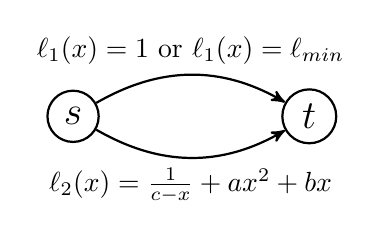
\begin{tikzpicture}
			\begin{scope}[->,>=stealth',auto,node distance=3cm,thick,main/.style={circle,draw,font=\sffamily\Large\bfseries}]				
				\node[main] (source) {$s$}; %
				\node[main, right of = source] (tail) {$t$}; %
				\draw [->] (source) to [in=150,out=30] node[above, align=center]{$\ell_1(x)=1$ or $\ell_1(x)=\ell_{min}$} (tail); %
				\draw [->] (source) to [in=-150,out=-30] node[below, align=center]{$\ell_2(x)=\frac{1}{c-x}+ax^2+bx$} (tail); %
			\end{scope}
		\end{tikzpicture}
	}%
	\caption{Worst-case network used to upper bound the price of anarchy.}
	\label{fig:poaexample}
\end{figure}

\pagebreak
\bibliographystyle{unsrtnat}
\bibliography{refs.bib}
\end{document}

